\setcounter{page}{1}
\section*{Zielsetzung}
Der Versuch US $1$ dient als Einführung in die Ultraschalltechnik.
Mit ihm sollen grundlegende physikalsische Eigenschaften der
Ultraschallechographie beobachtet und untersucht werden.
\section{Theorie}
\subsection{Schall und Schallausbreitung}
Liegt Schall in einem Frequenzbereich von $\SI{20}{\kilo\hertz}$ bis $\SI{1}{\giga\hertz}$,
wird als \emph{Ultraschall} bezeichnet. Er ist vom Menschen nicht wahrnehmbar.
Schall breitet sich als longitudinale Druckwelle $p(x,t)$ der Form
\begin{equation*}
  p(x,t)=p_0+v_0 Z \cos(\omega t - kx) \qquad Z=c\rho
\end{equation*}
aus. Die in der Gleichung auftretende Größe $Z$ bezeichnet die \emph{akustische Impendanz}.
Die Impendanz wird durch die Dichte $\rho$ des durchquerten Materials und der
materialabhängige Schallgeschwindigkeit festgelegt.
In Flüssigkeiten ist die Schallgeschwindigkeit abhängig von der
Kompressibilität $\kappa$ und der Flüssigkeitsdichte $\rho$
\begin{equation*}
  c\ua{Fl}=\sqrt{\frac{1}{\kappa\rho}}.
\end{equation*}
Statt der Kompressibilität hängt die Schallgeschwindigkeit in einem Festkörper von
dem Elastizitätsmodul $E$ ab:
\begin{equation*}
  c\ua{Fe}=\sqrt{\frac{E}{\rho}}.
\end{equation*}
Zusätzlich wird das Untersuchen von Schall im Festkörpern durch Schubspannungen
erschwert. Die Schubspannungen sorgen dafür, dass sich die Schallwelle nicht nur
Longlitudianle (wie zum Beispiel in Flüssigkeiten), sondern auch als
Transversalwellen ausbreiten.
Dazu kommt das die Schallgeschwindigeit in Festkörper eine Richtungsabhängigkeit
besitzt.
Ähnlich wie bei elektromagnetischen Wellen, können bei Schallwellen auch
Phänomene wie zum Beispiel Reflexion oder Brechung auftreten.

Wie bei mechanischen Wellen, gibt es bei Schallwellen dissipative Effekte.
Hierdurch verliert die Welle ein Teil der Energie bei Schallausbreitung:
\begin{equation}
  \label{eq:abfall}
  I(x)=I_0\map{e}^{-\alpha x}.
\end{equation}
Die Größe $\alpha$ ist der Absorptionskoeffizient der Schallamplitude und $I_0$ ist die
Intensität.
Besonders bei Luft ist $\alpha$ groß, deshalb wird immer ein Kontaktpotential
zwischen Schallgeber und zu untersuchendem Material verwendet.

Beim Auftrefen einer Schallwelle auf eine Grenzfläche, wird nur ein Teil der
Welle transmitiert. Der andere Teil wird reflektiert.
Ein Maß für die Reflexion bietet der Reflexionskoeffizient $R$.
Dieser gibt das Intensitätverhältnis zwischen einfallender und reflektierten Welle an.
Er kann mittels der in den anliegenden Materialien vorliegdenden Impendanzen $Z_1$ und $Z_2$
\begin{equation*}
  R=\left(\frac{Z_1-Z_2}{Z_1+Z_2}\right)^2
\end{equation*}
berechnet werden.
Der Transmittierte Anteil $T$ lässt sich mit $T=1-R$ ermitteln.

\subsection{Erzeugung und Empfangen von Ultraschall}

Eine Möglichkeit Ultraschallwellen zu erzeugen bietet der \emph{piezo-elektrischen Efffekt}.
Befindet sich ein \emph{piezoelektrischer} Kristall in einem elektrischenz Feld und steht
zusätzlich eine polare Achse des Krirstalles parrallel zum E-Feld, so wird dieser
zum Schwingen angeregt. Bei den abgestrahlten Wellen handelt es sich um Ultraschallwellen.
Insbesondere ist das erzeugen von Schwingungen mit hohen Schallenergiiendichten möglich,
wenn der Kristall mit seiner Resonanzfrequenz angeregt wird.
Neben dem Erzeugen bietet der piezoelektrischer Kristall auch die Möglichkeit
als Empfänger zu fungieren.

\subsection{Methoden der Ultraschallmessung}
Bei der Ultraschalluntersuchungen verwendet man das \emph{Durchschallungs-Verfahren} oder
das \emph{Impuls-Echo-Verfahren}.

Die schematische Darstellung des Durchschallungs-Verfahren ist in Abbildung
\ref{fig: durch} illustriert. Vor und hinter der Probe werden ein Ultraschallsender bzw. -empfänger
plaziert.
\begin{figure}[h]
  \centering
  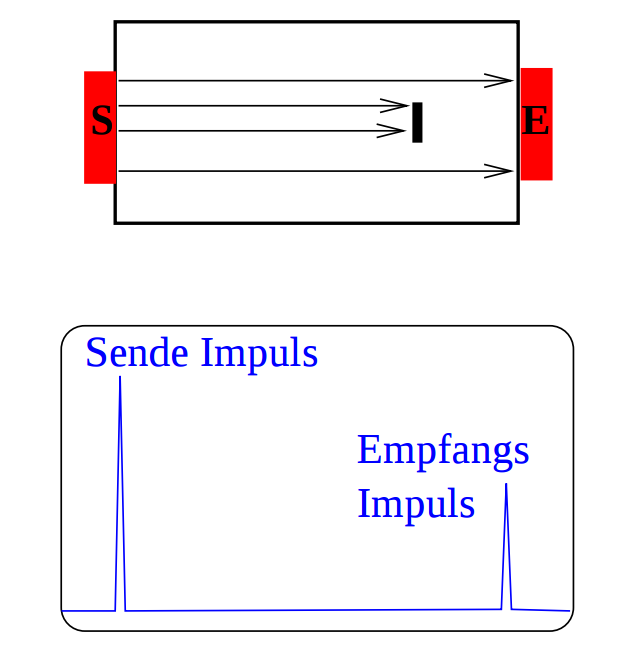
\includegraphics[width=0.4\textwidth]{pics/durchsall.png}
  \caption{Schematische Darstellung des Durchschallungs-Verfahren \cite{anleitungus1}.}
  \label{fig: durch}
  \end{figure}
Der Sender erzeugt kurzzeitige Schallimpulse, das vom Empfänger
regrestriert wird. Befindet sich eine Fehlstelle in der Probe, so misst der Empfänger
eine verringerte Intensität. Jedoch bietet dieses Verfahren keine Möglichkeit die
Fehlstelle zu lokalisieren.


Beim Impuls-Echo-Verfahren ist der Sender zeitgleich der Empfänger (vgl. Abb. \ref{fig: echo}).
\begin{figure}[h]
  \centering
  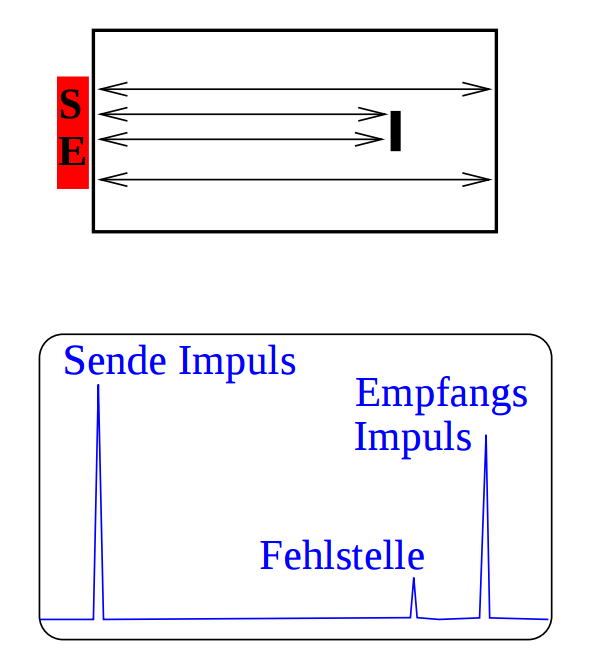
\includegraphics[width=0.4\textwidth]{pics/impuls_echo.png}
  \caption{Schematische Darstellung Impuls-Echo-Verfahren \cite{anleitungus1}.}
  \label{fig: echo}
  \end{figure}
Die erzeugte Schallwelle wird bei der Grenzfläche reflektiert und von der Sonde
empfangen. Mit Hilfe dieses Verfahren können auch die Orte der Fehlstellen bestimmt
werden. Ist die materialabhängige Schallgeschwindigkeit bekannt, so kann die
Lage der Fehlstelle mit
\begin{equation}
  \label{eq:lage_fehl}
  s=\frac{1}{2}ct
\end{equation}
bestimmt werden.

Um die Ergebnisse einer Ultraschallmessung zu veranschaulichen, werden drei verschiedene
Darstellungsmöglichkeiten verwendet.

Eine Möglichkeit bietet der \emph{A-Scan} (A für Amplitude), in diesem
wird die Zeit gegen die empfangenen Amplitude aufgetragen.
Ein beispielhafter Verlauf ist in Abbildung \ref{} dargestellt.

Neben dem \emph{A-Scan} gibt es noch den \emph{B-Scan} (B für Brightness).
Bei einem B-Scan wird die Größe der gemessene Amplitude als Heligkeit
angegeben. Dadurch ist es möglich ein 2 dim. Bild von der Probe zu erzeugen.

Abschließend bietet der \emph{TM-Scan} (TM bedeutet time motion) die Möglichkeit
Bewegungen in der zu untersuchende Probe darzustellen.
